\documentclass[10pt,a4paper]{article}
\usepackage[margin=2.3cm]{geometry}
\usepackage[T1]{fontenc}
\usepackage{lmodern}
\usepackage{amsmath,amssymb}
\usepackage{graphicx}
\usepackage{booktabs,tabularx,array,longtable}
\usepackage{xcolor}
\usepackage{listings}
\usepackage{tikz}
\usetikzlibrary{arrows.meta,positioning}
\usepackage{enumitem}
\usepackage{caption}\usepackage{tocloft}
\usepackage[hidelinks]{hyperref}
\setlist{nosep,leftmargin=1.4em}\setcounter{tocdepth}{1}\setlength{\cftbeforesecskip}{1pt}\setlength{\cftbeforesubsecskip}{0pt}
\newcommand{\fn}[1]{\texttt{\detokenize{#1}}}
\newcolumntype{L}{>{\raggedright\arraybackslash}X}
\definecolor{codebg}{RGB}{246,246,246}
\lstset{language=Python,basicstyle=\ttfamily\footnotesize,backgroundcolor=\color{codebg},
  frame=single,rulecolor=\color{gray!40},columns=fullflexible,keepspaces=true,showstringspaces=false,
  keywordstyle=\color{blue!60!black},commentstyle=\color{green!40!black},stringstyle=\color{red!50!black},
  breaklines=true,xleftmargin=2pt,xrightmargin=2pt}

\title{PCB Defect Detection Under Image Misalignment\\[2pt]
\large Data Preparation Report --- COEN 6314 Course Project}
\author{Basma Kurany \quad (ID 40374114)\\ \small Concordia University, Gina Cody School of Engineering and Computer Science}
\date{October 2026}

\begin{document}
\maketitle

\begin{abstract}
This report summarizes DeepPCB and the reproducible preparation pipeline for studying PCB defect detection under image misalignment. It covers the source audit, grouped split, controlled shifts, label handling, verification, and model-ready exports. Proposal V4 lists Fast R-CNN, YOLOv10-Nano, and SSD-MobileNet as detector options. This project selects YOLOv10-Nano for the implementation. This report presents preparation results only, not model performance.
\end{abstract}

\tableofcontents
\newpage

%=====================================================================
\section{Data and source: DeepPCB}
DeepPCB~\cite{tang2019} contains 1,500 pairs of $640\times640$ template and inspected images with bounding boxes for six defect classes: open, short, mousebite, spur, copper, and pin-hole. The images were cropped from larger board scans and aligned by template matching. Most defects were artificially added by the dataset authors, so performance on real production defects may differ.

Each source pair has a reference JPEG, an inspected JPEG, and a text label file containing \fn{x1 y1 x2 y2 class}. The official \fn{trainval.txt} and \fn{test.txt} lists define the retained 1,000/500 pair partition. The extracted source data are under \fn{Data/DeepPCB-master/DeepPCB-master/PCBData/}.

\begin{table}[h]
\centering\small
\caption{Raw pair and annotation counts.}
\begin{tabular}{@{}lrrrrrrr@{}}
\toprule
Split & Pairs & Open & Short & Mousebite & Spur & Copper & Pin-hole \\
\midrule
Trainval & 1,000 & 1,283 & 1,028 & 1,379 & 1,142 & 1,010 & 1,031 \\
Test & 500 & 659 & 478 & 586 & 483 & 464 & 470 \\
Total & 1,500 & 1,942 & 1,506 & 1,965 & 1,625 & 1,474 & 1,501 \\
\bottomrule
\end{tabular}
\end{table}
There are 10,013 boxes (1--15 per pair; median 7). Box widths range from 18 to 173 px (median 35); heights range from 19 to 152 px (median 33). The source contains 11 groups; four groups absent from trainval account for 332 test pairs. Fifty-seven pairs contain at least one 3-channel JPEG; all prepared outputs are grayscale PNGs.

\section{Preparation pipeline}
The pipeline indexes and audits the source, selects validation groups, generates deterministic shifted sets, checks image/label geometry, then exports COCO and YOLO formats. It leaves source data unchanged. Seed 6314 is combined with each pair ID so transformations do not depend on file order.

\begin{table}[h]
\centering\small
\caption{Preparation scripts and outputs.}
\begin{tabularx}{\linewidth}{@{}lL@{}}
\toprule
Scripts & Role \\
\midrule
\fn{01_inspect.py}, \fn{02_duplicates_alignment.py}, \fn{03_verify_dups_alignment.py} & Index source files, find near-duplicate candidates, and audit native alignment. \\
\fn{04_make_splits.py} & Create group-aware train/validation/test manifests and duplicate flags. \\
\fn{05_make_shift_sets.py}, \fn{pcb_shift.py} & Generate fixed evaluation conditions and transformed boxes; provide training jitter utilities. \\
\fn{06_qa_checks.py} & Run geometry checks and produce visual check sheets. \\
\fn{07_export_coco.py}, \fn{08_make_yolo.py}, \fn{09_check_yolo.py} & Export model-ready annotations/images and verify the YOLO package. \\
\fn{run_all.sh} & Run the pipeline from the raw DeepPCB folder. \\
\bottomrule
\end{tabularx}
\end{table}
The implementation currently provides a YOLOv10-Nano input pipeline. YOLOv10-Nano is one of the compact detectors listed in Proposal V4; the three-channel composite gives it both images as input, as the proposal requires. The preparation pipeline itself uses Python, NumPy, and OpenCV; Ultralytics is used in the subsequent training stage.

\section{Audit and partition design}\label{sec:audit}
\subsection{Native alignment and duplicate pairs}
An integer translation is estimated by minimizing template/inspection XOR disagreement over offsets up to $\pm8$ px. A pair is flagged when the best non-zero offset reduces disagreement by at least 1.5 times. This heuristic finds 123/1,500 natively misaligned pairs (75 train, 8 validation, 40 test), with offsets up to 8 px. Thus \fn{s0} means “as supplied,” not guaranteed perfect alignment.

\begin{figure}[h]
\centering
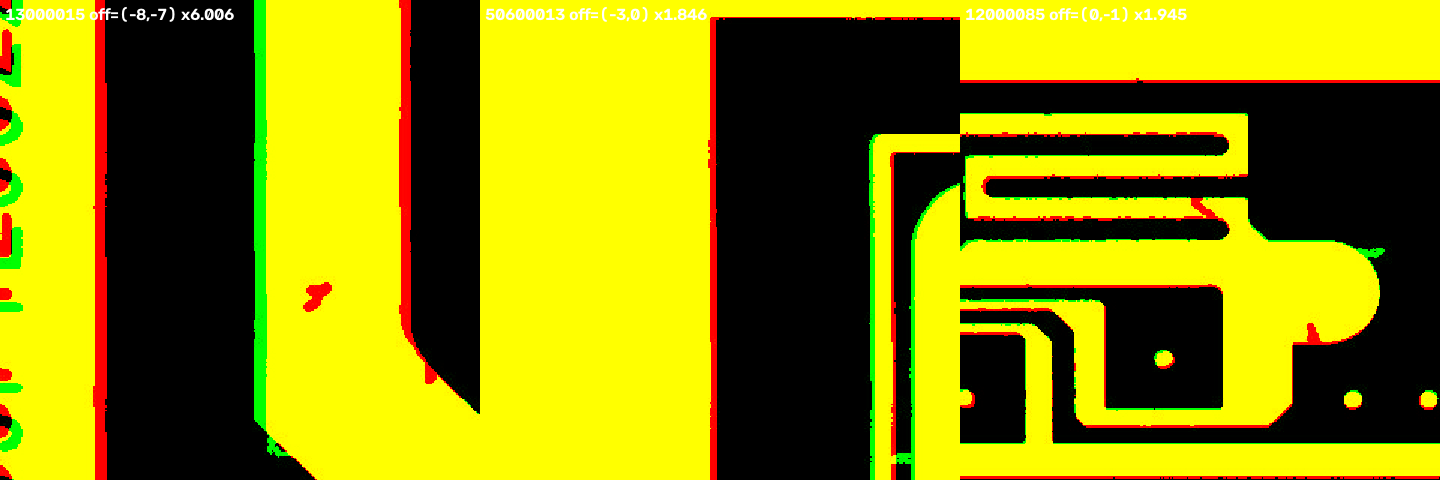
\includegraphics[width=0.9\linewidth]{fig/native_misalignment_examples.png}
\caption{Examples of native misalignment. Red and green show pixels unique to each image; yellow shows overlap.}
\label{fig:native}
\end{figure}

A dHash scan produced 337 candidates, followed by pixel-level comparison after shifts up to 8 px. Forty duplicate pairs were confirmed, all within the same source group. Three test pairs (50600065, 92000114, 92000118) duplicate training pairs and are flagged for a separate sensitivity analysis.

\subsection{Grouped split}
The official 500-pair test set is retained. One whole trainval group, group00041 (200 pairs), is held out for validation; the remaining 800 pairs form training data. This keeps transformed copies together and approximates the test set’s unseen-group setting. The group choice minimizes the $L_1$ difference in class proportions among candidate group-held-out splits between 17\% and 23\% of trainval.

\begin{table}[h]
\centering\small
\caption{Final partition sizes and group assignment.}
\begin{tabularx}{\linewidth}{@{}lrrL@{}}
\toprule
Split & Pairs & Native-offset pairs & Groups \\
\midrule
Train & 800 & 75 & 13000, 20085, 44000, 50600, 77000, 92000 \\
Validation & 200 & 8 & 00041 \\
Test & 500 & 40 & all 11 official test groups \\
\bottomrule
\end{tabularx}
\end{table}
The primary result should use all 500 official test pairs. A clean-pair sensitivity analysis may exclude the 40 natively misaligned test pairs, leaving 460 test pairs; 1,377 is the clean count across the full 1,500-pair dataset, not the test-set size.

\section{Controlled misalignment and labels}\label{sec:shifts}
Validation and test each contain ten conditions: the supplied pair (\fn{s0}); horizontal and vertical shifts of 1, 2, 3, and 5 px (eight conditions); and a residual condition with a 0.25--1.5 px translation plus rotation in $[-0.5^\circ,0.5^\circ]$. Training stores only the 800 \fn{s0} images; augmentation is generated separately. Every transform is seeded per pair and shared by the inspected image and its boxes, while the reference remains fixed. Integer shifts use exact pixel sampling; residual transforms use bilinear interpolation.

For rotations, the four box corners are transformed and enclosed by a tight axis-aligned box. A padded 8 px border is excluded at evaluation. Boxes within 14 px of an original image edge are marked ignore consistently across conditions (258/10,013 boxes, 2.6\%). These annotations should be treated as “don’t care” during evaluation.

\begin{figure}[p]
\centering
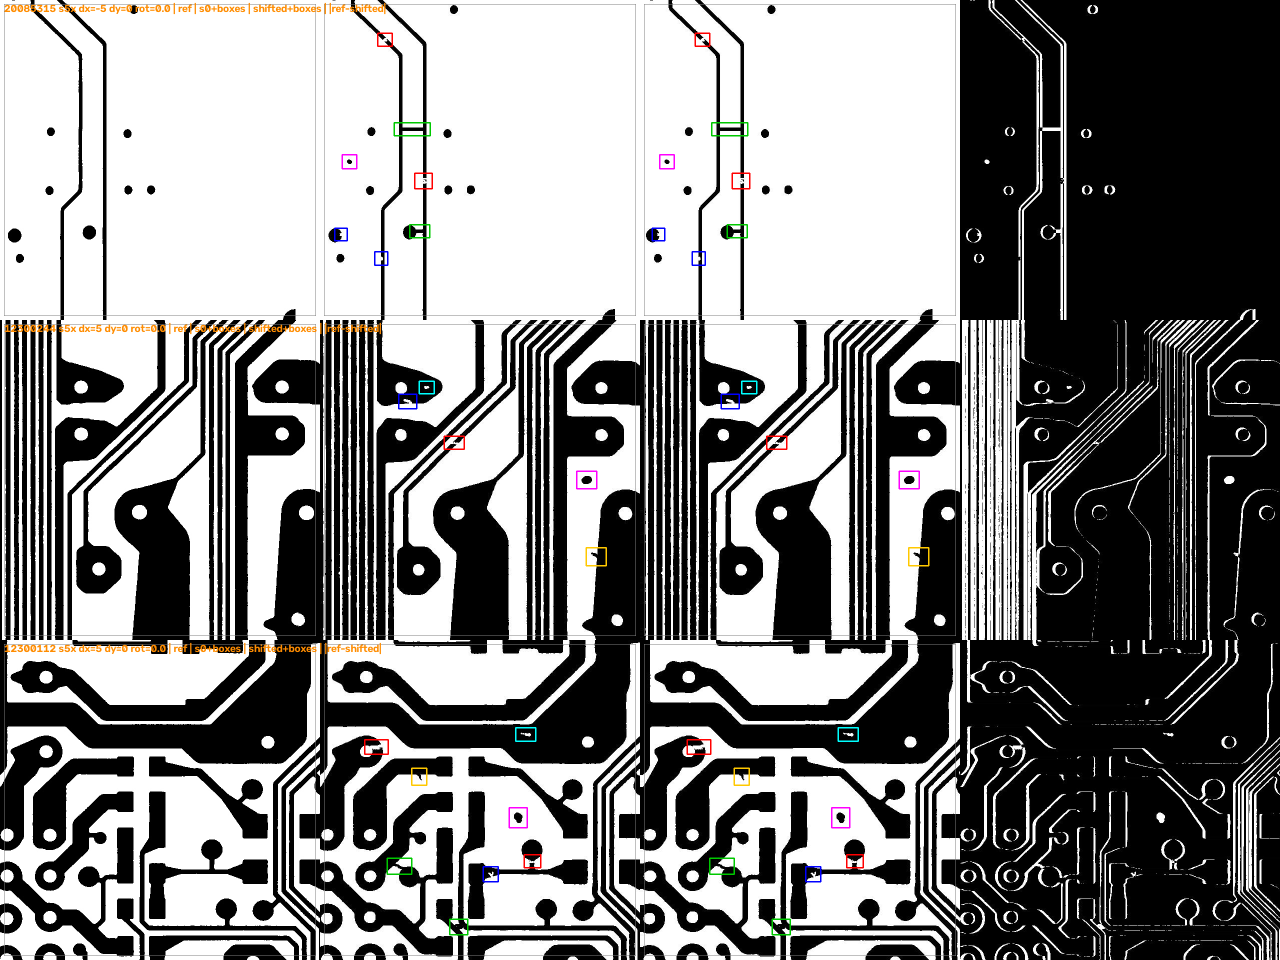
\includegraphics[width=\linewidth]{fig/check_s5x.png}\\[2mm]
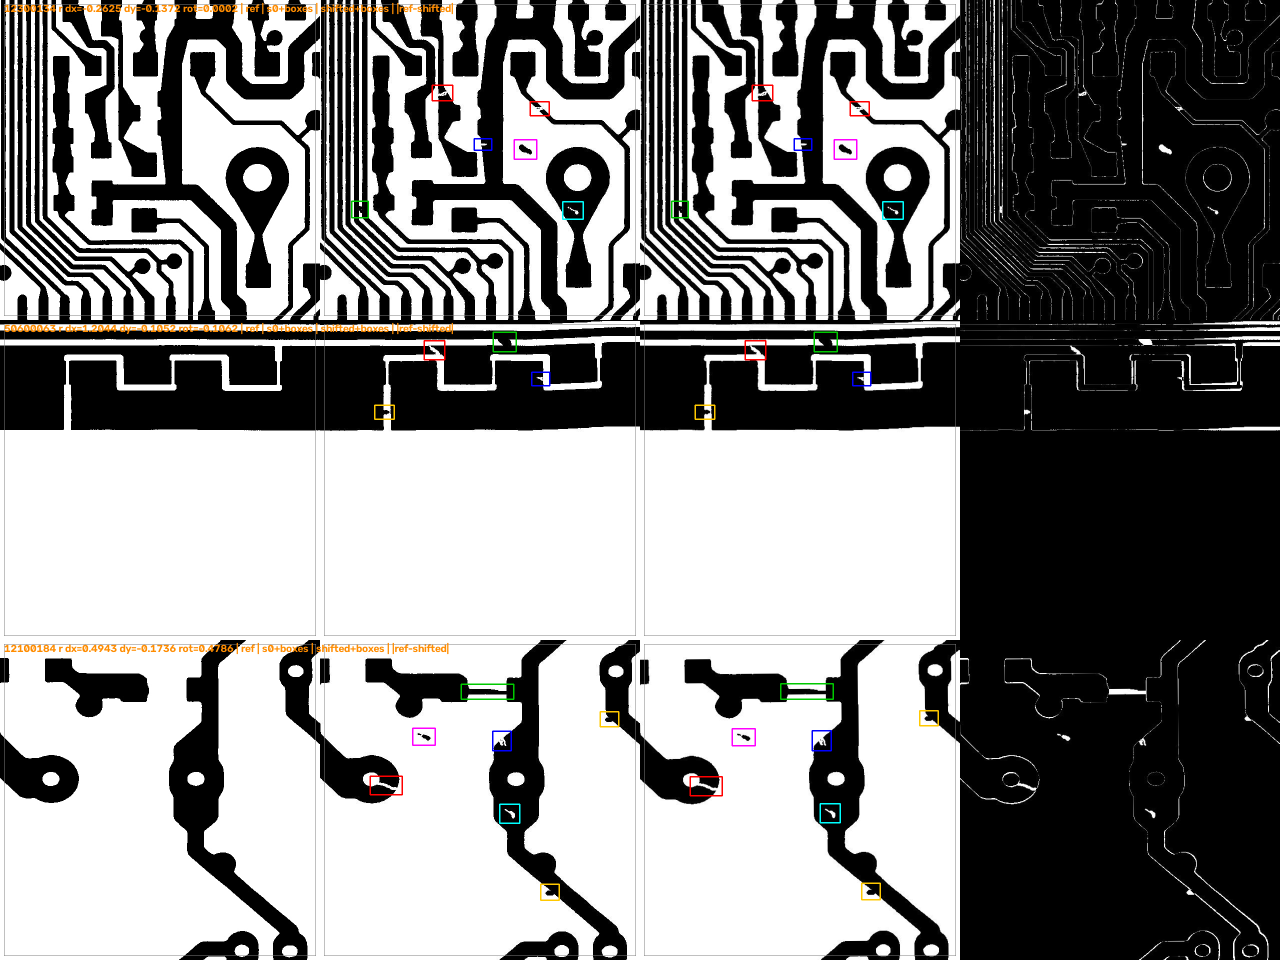
\includegraphics[width=\linewidth]{fig/check_r.png}
\caption{Visual checks for a 5 px shift (top) and residual transform (bottom). Columns show the reference, original inspected image with boxes, transformed image with boxes, and absolute difference.}
\end{figure}


\section{Data exports and model input}
The manifests preserve pair IDs, groups, splits, condition parameters, paths, transformed boxes, class IDs, and ignore flags. CSV is the audit-friendly master format; COCO provides one JSON per split/condition (21 files). The source label text files remain unchanged. YOLO exports use one normalized \fn{class xc yc w h} row per box and a three-channel composite: reference, inspected image, and absolute difference.

\begin{table}[h]
\centering\small
\caption{Main generated artifacts.}
\begin{tabularx}{\linewidth}{@{}lL@{}}
\toprule
Artifact & Contents \\
\midrule
\fn{sets/ref/} & 1,500 unchanged reference PNGs. \\
\fn{sets/<split>/<condition>/} & 7,800 grayscale inspection PNGs. \\
\fn{index/pairs.csv}, \fn{boxes.csv}, \fn{splits.csv} & Source inventory, annotations, and partition metadata. \\
\fn{index/images.csv}, \fn{labels.csv} & Per-image transform metadata and per-box labels/ignore flags. \\
\fn{index/coco/} & COCO exports for each available split/condition. \\
\fn{yolo_train.zip}, \fn{yolo_eval_*.zip} & YOLO training and evaluation composites with labels. \\
\fn{reports/}, \fn{qa/} & Machine-readable summaries and visual checks. \\
\bottomrule
\end{tabularx}
\end{table}

The YOLO training package contains an 800-pair unaugmented set and a 2,400-image augmented set (original, one random integer shift, and one residual transform per pair). Colour-channel augmentation is disabled because independent channel changes would corrupt the difference channel. YOLO labels cannot encode the ignore flag; the project’s evaluation must read the master CSV and apply the ignore rule itself.

\begin{figure}[h]
\centering
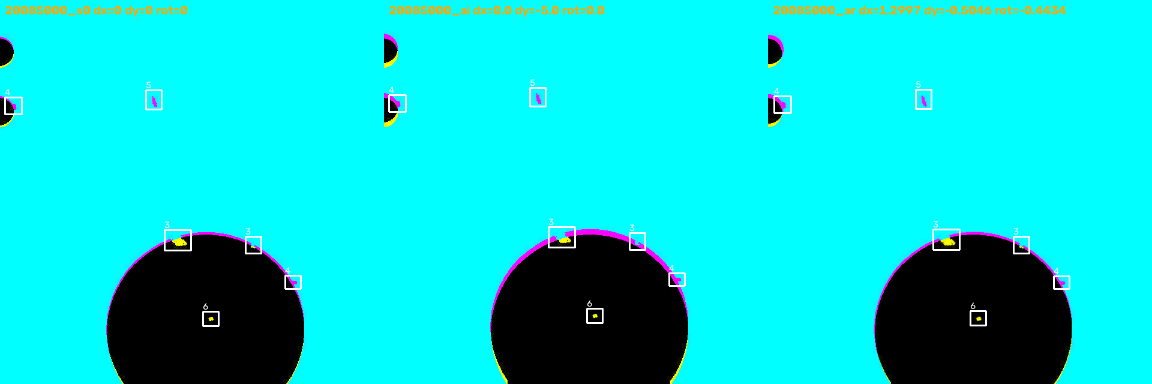
\includegraphics[width=0.88\linewidth]{fig/yolo_check.png}
\caption{YOLO export check for the original, shifted, and residual versions of one pair.}
\end{figure}

\section{Verification and use}
\begin{table}[h]
\centering\small
\caption{Automated preparation checks.}
\begin{tabularx}{\linewidth}{@{}Lr@{}}
\toprule
Check & Result \\
\midrule
Integer-shift pixel checks & 5,600/5,600 passed \\
Transformed box-content checks & 36,640/36,640 passed \\
Non-ignored boxes inside valid region & 41,220/41,220 passed \\
Residual transform audit (120 samples) & Median corner error 0.002 px; max 0.05 px \\
YOLO labels present with matching counts/classes & 10,200/10,200 passed \\
Composite channel construction (342 samples) & 342/342 passed \\
\bottomrule
\end{tabularx}
\end{table}
The YOLO round-trip check reports coordinate differences for ignored boxes clipped at image boundaries. Evaluation should continue to use the un-clipped master annotations and apply the documented ignore rule.

To rebuild the preparation outputs, install Python 3, NumPy, and OpenCV, set \fn{PCB_ROOT} to the extracted \fn{PCBData} directory if it is not at the documented default, then run \fn{bash MyData/scripts/run_all.sh}. YOLO training uses Ultralytics in Colab; the exported YAML files point to the unaugmented and augmented training sets. Select thresholds on validation data only and evaluate the official test set once.

\section{Limitations and next steps}
The data have four main limitations: many defects are synthetic; 123 pairs have native alignment offsets; validation consists of one source group; and each validation/test pair has only one residual variant. Three confirmed train/test duplicate pairs also warrant a separately labeled sensitivity result. These constraints should accompany model-performance claims.

Next, implement the registered and unregistered differencing baselines, train aligned-only and jitter-trained YOLO models, tune the common target-recall threshold on validation, and compare results on the full official test set with a 460-pair clean-test sensitivity analysis.

\begin{thebibliography}{9}
\bibitem{tang2019} S.~Tang, F.~He, X.-L.~Huang, and J.~Yang, ``Online PCB defect detector on a new PCB defect
dataset,'' \emph{arXiv:1902.06197}, 2019.
\end{thebibliography}
\end{document}

